% cd /storage/emulated/0/Documents/documents/latex/1920/Grade-10/tests/ && pdflatex Sir-gen-quiz-bee.tex && termux-open Sir-gen-quiz-bee.pdf

\documentclass[12pt,letterpaper]{article}
\usepackage[utf8]{inputenc}
\usepackage{xcolor}
\usepackage{anyfontsize}
\usepackage{enumitem}
\usepackage{multicol}
\usepackage{amsmath}
\usepackage{gensymb}
\usepackage{multirow}
\usepackage{graphicx, tipa}
\usepackage{tikz}
\usetikzlibrary{angles,quotes}
\usepackage{pgfplots} 
\usetikzlibrary{calc}
\pgfplotsset{compat=newest}
\usetikzlibrary{arrows.meta}
\usetikzlibrary{intersections}
\usetikzlibrary{decorations.pathreplacing}


\def\radA{4cm}

\def\radB{2.5cm}

\usepackage[left=2.3cm,right=1.5cm,top=1.5cm,bottom=1.5cm]{geometry}

\begin{document}
\begin{center}
\textbf{SEARCH FOR THE MATHEMATICIAN OF THE YEAR}\\
Sauyo High School\\
2019 - 2020
\end{center}
\noindent NAME: \underline{\hspace{5.6cm}} \hfill DATE: \underline{\hspace{3cm}}
\\
\noindent SECTION: \underline{\hspace{5cm}} \hfill SCORE: \underline{\hspace{2.75cm}}
\\
INSTRUCTION: Solve each problem and write only your answer before each number. Express answers in lowest terms.
\begin{enumerate}
%1
\item[\underline{\hspace{1.5cm}}1.] Simplify $\sqrt{32}$.
%2
\item [\underline{\hspace{1.5cm}}2.]What is the vertex of the quadratic function $y=(x-4)^2+5$?   
%3
\item [\underline{\hspace{1.5cm}}3.]If $4$ men can do a job in $20$ days, in how many days can $5$ men finish the same job?
%4
\item [\underline{\hspace{1.5cm}}4.]Solve for $x$ in the quadratic equation $x^2+3x-10=0$.
%5
\item [\underline{\hspace{1.5cm}}5.]Betty has $5$ daughters and no sons. Some of her daughters have $5$ daughters and the rest have none. Betty has a total of $25$ daughters and granddaughters and no great granddaughters. How many of Betty's daughters and granddaughters have no daughters?
%6
\item [\underline{\hspace{1.5cm}}6.]Find a quadratic equation in form $ax^2+bx+c=0$ whose roots are $7$ and $-2$.
%7
\item [\underline{\hspace{1.5cm}}7.]What is the discriminant value of the quadratic $4x^2+12x+9=0$?
%8
\item [\underline{\hspace{1.5cm}}8.]What is the sum of the roots of the quadratic equation $20x^2+19x+21=0$?
%9
\item [\underline{\hspace{1.5cm}}9.]If $y$ varies directly as $x$ and $y=15$ when $x=9$, find $y$ when $x=12$.
%10
\item [\underline{\hspace{1.3cm}}10.]James and George goes to the barbershop every $12$ days and $9$ days, respectively. Last time they met was a Tuesday. What day of the week will it be the next time they meet?
%11
\item [\underline{\hspace{1.3cm}}11.]In figure $\#1$, $line\ m \parallel line\ n$. Find the value of $x$.
\\
\begin{center}
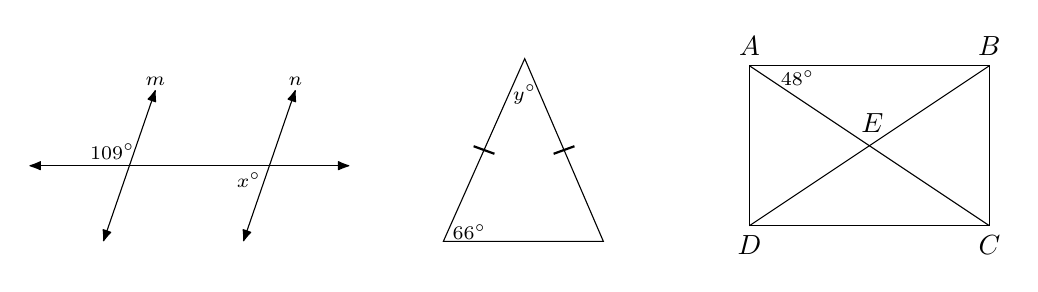
\begin{tikzpicture}

\coordinate (a) at (0,0);
\coordinate (b) at (0.7in,0);
\coordinate (c) at ($(a)+(71:0.4in)$);
\coordinate (d) at ($(b)+(71:0.4in)$);
\coordinate (e) at ($(a)+(-109:0.4in)$);
\coordinate (f) at ($(b)+(-109:0.4in)$);

\draw [<->, >={Latex[round]}](-0.5 in,0)--(a)--(b)--(1.1 in,0);
\draw [<->, >={Latex[round]}](c)--(e);
\draw [<->, >={Latex[round]}](d)--(f);

\node (109) at ($(a)+(140:8pt)$){$\scriptstyle 109 \degree $};
\node (x) at ($(b)+(215:9pt)$){$\scriptstyle x \degree$};
\node (m) at($(c)+(90:3pt)$){$\scriptstyle m$};
\node (m) at($(d)+(90:3pt)$){$\scriptstyle n$};

\coordinate (g) at ($(f)+(0:1in)$);
\coordinate (h) at ($(g)+(0:0.8in)$);
\coordinate (i) at ($(g)+(66:1in)$);

\node (g.label) at ($(g)+(20:10pt)$){$\scriptstyle 66\degree$};

\node (i.label) at ($(i)+(-90:13pt)$){$\scriptstyle y \degree$};
\draw (g)--(h)--node[midway] (tick2) {}(i)--node[midway] (tick1) {}cycle;

\tikzset{onetick/.pic={\draw[thick] ($(0,0)+(0,4pt)$) -- ($(0,0)-(0,4pt)$) ; }}

\pic[rotate=70] at (tick1) [pic type = onetick];

\pic[rotate=-70] at (tick2) [pic type = onetick];

\coordinate (x) at (3.1in,-0.3in);
\coordinate (y) at (4.3in,-0.3in);
\coordinate (z) at (4.3in, 0.5in);
\coordinate (w) at (3.1in,0.5in);

\draw (x)--(y)--(z)--(w)--cycle;
\draw (x)--(z);
\draw (y)--(w);

\node (D.label) at ($(x)+(-90:7pt)$){$\displaystyle D$};
\node (C.label) at ($(y)+(-90:7pt)$){$\displaystyle C$};
\node (B.label) at ($(z)+(90:7pt)$){$\displaystyle B$};
\node (A.label) at ($(w)+(90:7pt)$){$\displaystyle A$};
\node (E.label) at ($(x)+(40:58pt)$){$\displaystyle E$};
\node (SDF.label) at ($(w)+(-14:18pt)$){$\scriptstyle 48 \degree$};
\end{tikzpicture}
\end{center}

\hspace{3cm} figure \#1 \hspace{2.5cm} figure \#2\hspace{2.5cm}   figure \#3
%12
\item [\underline{\hspace{1.3cm}}12.]In figure \# 2, find the value of $y$.
%13
\item [\underline{\hspace{1.3cm}}13.]In figure \# 3, $ABCD$ is a rectangle and $\angle BAC=48\degree$. Find $\angle DEC$. 
%14
\item 	[\underline{\hspace{1.3cm}}14.]Simplify the radical expression $\sqrt{8m^3n^4p^5}$.
%15
\item[\underline{\hspace{1.3cm}}15.] Elena is $24$ years old while her daughter is $3$ years old. In how many years will Elena be twice as old as her daughter?
%16
\item [\underline{\hspace{1.3cm}}16.]Solve for $x$: $\sqrt{3-x}=8$
%17
\item [\underline{\hspace{1.3cm}}17.]Solve the system: 
\begin{eqnarray*}
x-y&=&14\\
3x+y&=&2
\end{eqnarray*}
%18
\item [\underline{\hspace{1.3cm}}18.]Evaluate $\sqrt{18}+\sqrt{8}$
%19
\item [\underline{\hspace{1.3cm}}19.]A $13-ft$ ladder is leaning against a wall. If the foot of the ladder is $5\ ft$ away from the wall, how high up the wall does the ladder reach?
%20 
\item [\underline{\hspace{1.3cm}}20.]A worm is slowly crawling to the top of a pole $70\ m$ high. During the day it advances $7\ m$ and during the night it slips down $4\ m$. After how many days will it finally reach the top?				
%21
\item [\underline{\hspace{1.3cm}}21.]$ABCD$ is a trapezoid with $M$ and $N$ as the midpoints of the legs $AD$ and $BC$. If $AB=27$ and $CD=73$, how long is $MN$? 
%22
\item [\underline{\hspace{1.3cm}}22.]Find a quadratic equation whose roots are $3\pm \sqrt{17}$.	
%23
\item [\underline{\hspace{1.3cm}}23.]$ABCD$ is a rectangle. Its diagonals meet at $O$. If $AO=2x-3$ and $OB=x+5$, find $BD$.
%24
\item [\underline{\hspace{1.3cm}}24.]If $2^{2019}+2^{2019}=2^x$ , what is the value of $x$?
%25
\item [\underline{\hspace{1.3cm}}25.]What is the perimeter of a parallelogram $ABCD$ if $AB=4x+5$, $DC=2x+7$ and $AD=5x-1$.
%26
\item [\underline{\hspace{1.3cm}}26.]$\triangle ABC \sim \triangle XYZ$. If $AB=9\ cm$, $XY=15\ cm$ and $AC=6\ cm$, find $XZ$.
%27
\item [\underline{\hspace{1.3cm}}27.]Rolly drives $500\ km$ from his office to a business convention. On the return trip, he increases his speed by $25\ kph$ and saves $1$ hour of driving time. What is his speed in going to the convention?
%28
\item [\underline{\hspace{1.3cm}}28.]Find the solution set of $x^2+5x-24>0$ and write your answer in interval notation.
%29
\item [\underline{\hspace{1.3cm}}29.]How many rectangles can you count in the given figure?
\\
\begin{center}

\begin{tikzpicture}
\draw[step=1cm] (0,0)grid( 5cm,4cm);
\end{tikzpicture}
\end{center}

\item [\underline{\hspace{1.3cm}}30.] If a ship has $26$ sheep and $10$ goats onboard, how old is the ship's captain?
 
\end{enumerate}


\vspace{1cm}
\begin{small}“The greatest mathematics has the simplicity and inevitableness of supreme poetry and music, standing on the borderline of all that is wonderful in science and all that is beautiful in art. Mathematics transfigures the fortuitous concourse of atoms into the tracery of the the fingers of God." - H.W. Turnbull
\end{small}


\end{document}